%%%%%%%%%%%%%%%%%%%%%%%%%%%%%%%%%%%%%%%%%%%%%%%%%
%       Macroscopic analysis of load curve      %
%   Antoine                                     %
%%%%%%%%%%%%%%%%%%%%%%%%%%%%%%%%%%%%%%%%%%%%%%%%%
\subsection{Macroscopic analysis of load curve}

We need a fast algorithm that can be called at every moment to detect a device from the load curve. In that way, we develop algorithms based on a macroscopic approach, and if doubts appear we erase them with the microscopic algorithms.

The macroscopic algorithms are based on the differenciate function, it is easier to detect a jump in the load curbe with such a function. Indeed the difference between two point of a jump is directly the consumption of the device, as shown in \ref{fig1}.

\begin{figure}[H]
\centering
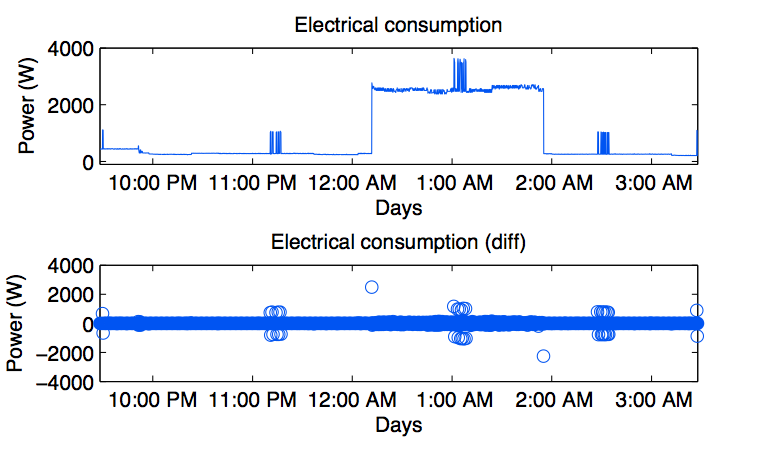
\includegraphics[scale=0.5]{figures/fig_antoine_5.png}
\caption{Example of a real load curve}
\label{fig1}
\end{figure}

We define several step of consumption: 100, 500 and 750W which mean for small consulption device (such as lights), medium consumption (oven) and eavy consumption (heater). Each time, the load curve reaches such a value, the device turns on, when the load curbe reach the same value negatively, the device turns off. With this basic approach we can define some devices, but we cannot differenciate an unknow device which consumes 500W from a oven for example.

So, we developped a second algorithm that analyze the signature load curve of each device. Every devices have a specific and unic load curve when they turn on and if we can create a data base with these signatures, then we can determine which device has just turn on. The time when they turn off is easy to spot because it is when the value of the differenciate function are negative.

Let us take an example to precise our idea. We simulated heater power consumption, which is basically a square repetition, because a heater is a periodical device. By detecting such a wave form in the load curve, then we can detect heater consumption and estimate the consumption of this device. Finally, we proceed with the same algorithms on real signal and we obtain the result shown on the figure \ref{fig2}.


\begin{figure}[H]
\centering
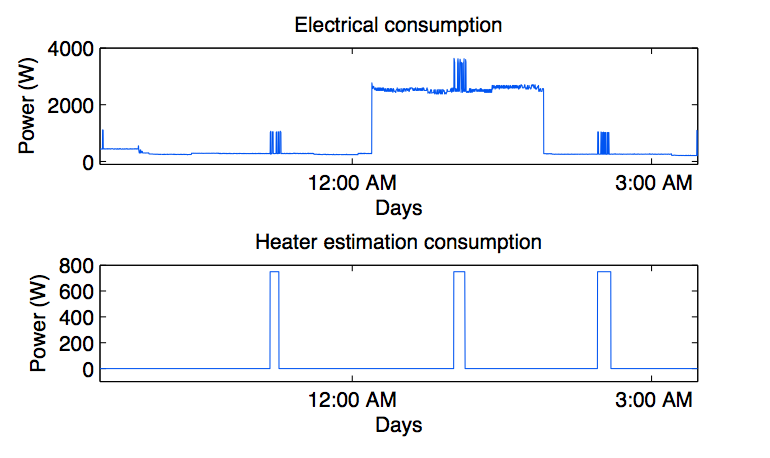
\includegraphics[scale=0.5]{figures/fig_antoine_6.png}
\caption{Estimation of a heater consumption}
\label{fig2}
\end{figure}


We proceed in the same way for non periodical devicces such as a dishwasher or a washing machine. But for instant, only the dishwasher is implemented.


